\chapter{Umsetzung}
\doublespacing
\section{Kommunikation zwischen ScanDriver und DK App}
\subsection{LMS4K ScanDiver}
Vermerk: Hier wird stehen welche Aufgabe welches File im ScanDriver hat. Hier ist zu sehen wie es dargestellt werden soll

\begin{description}
\item[EventHandlerMessage.lua]\hfill \\
Erzeugt die Funktion Message.Send die in drei Typen unterteilt sind ERROR , INFO  und WARNING. Es können die letzten 10 Nachrichten gespeichert werden. 
\end{description}

\subsection{DK App}
Vermerk: Hier wird stehen welche Aufgabe welches File im DK App hat




\begin{figure}[h!]
%\centering
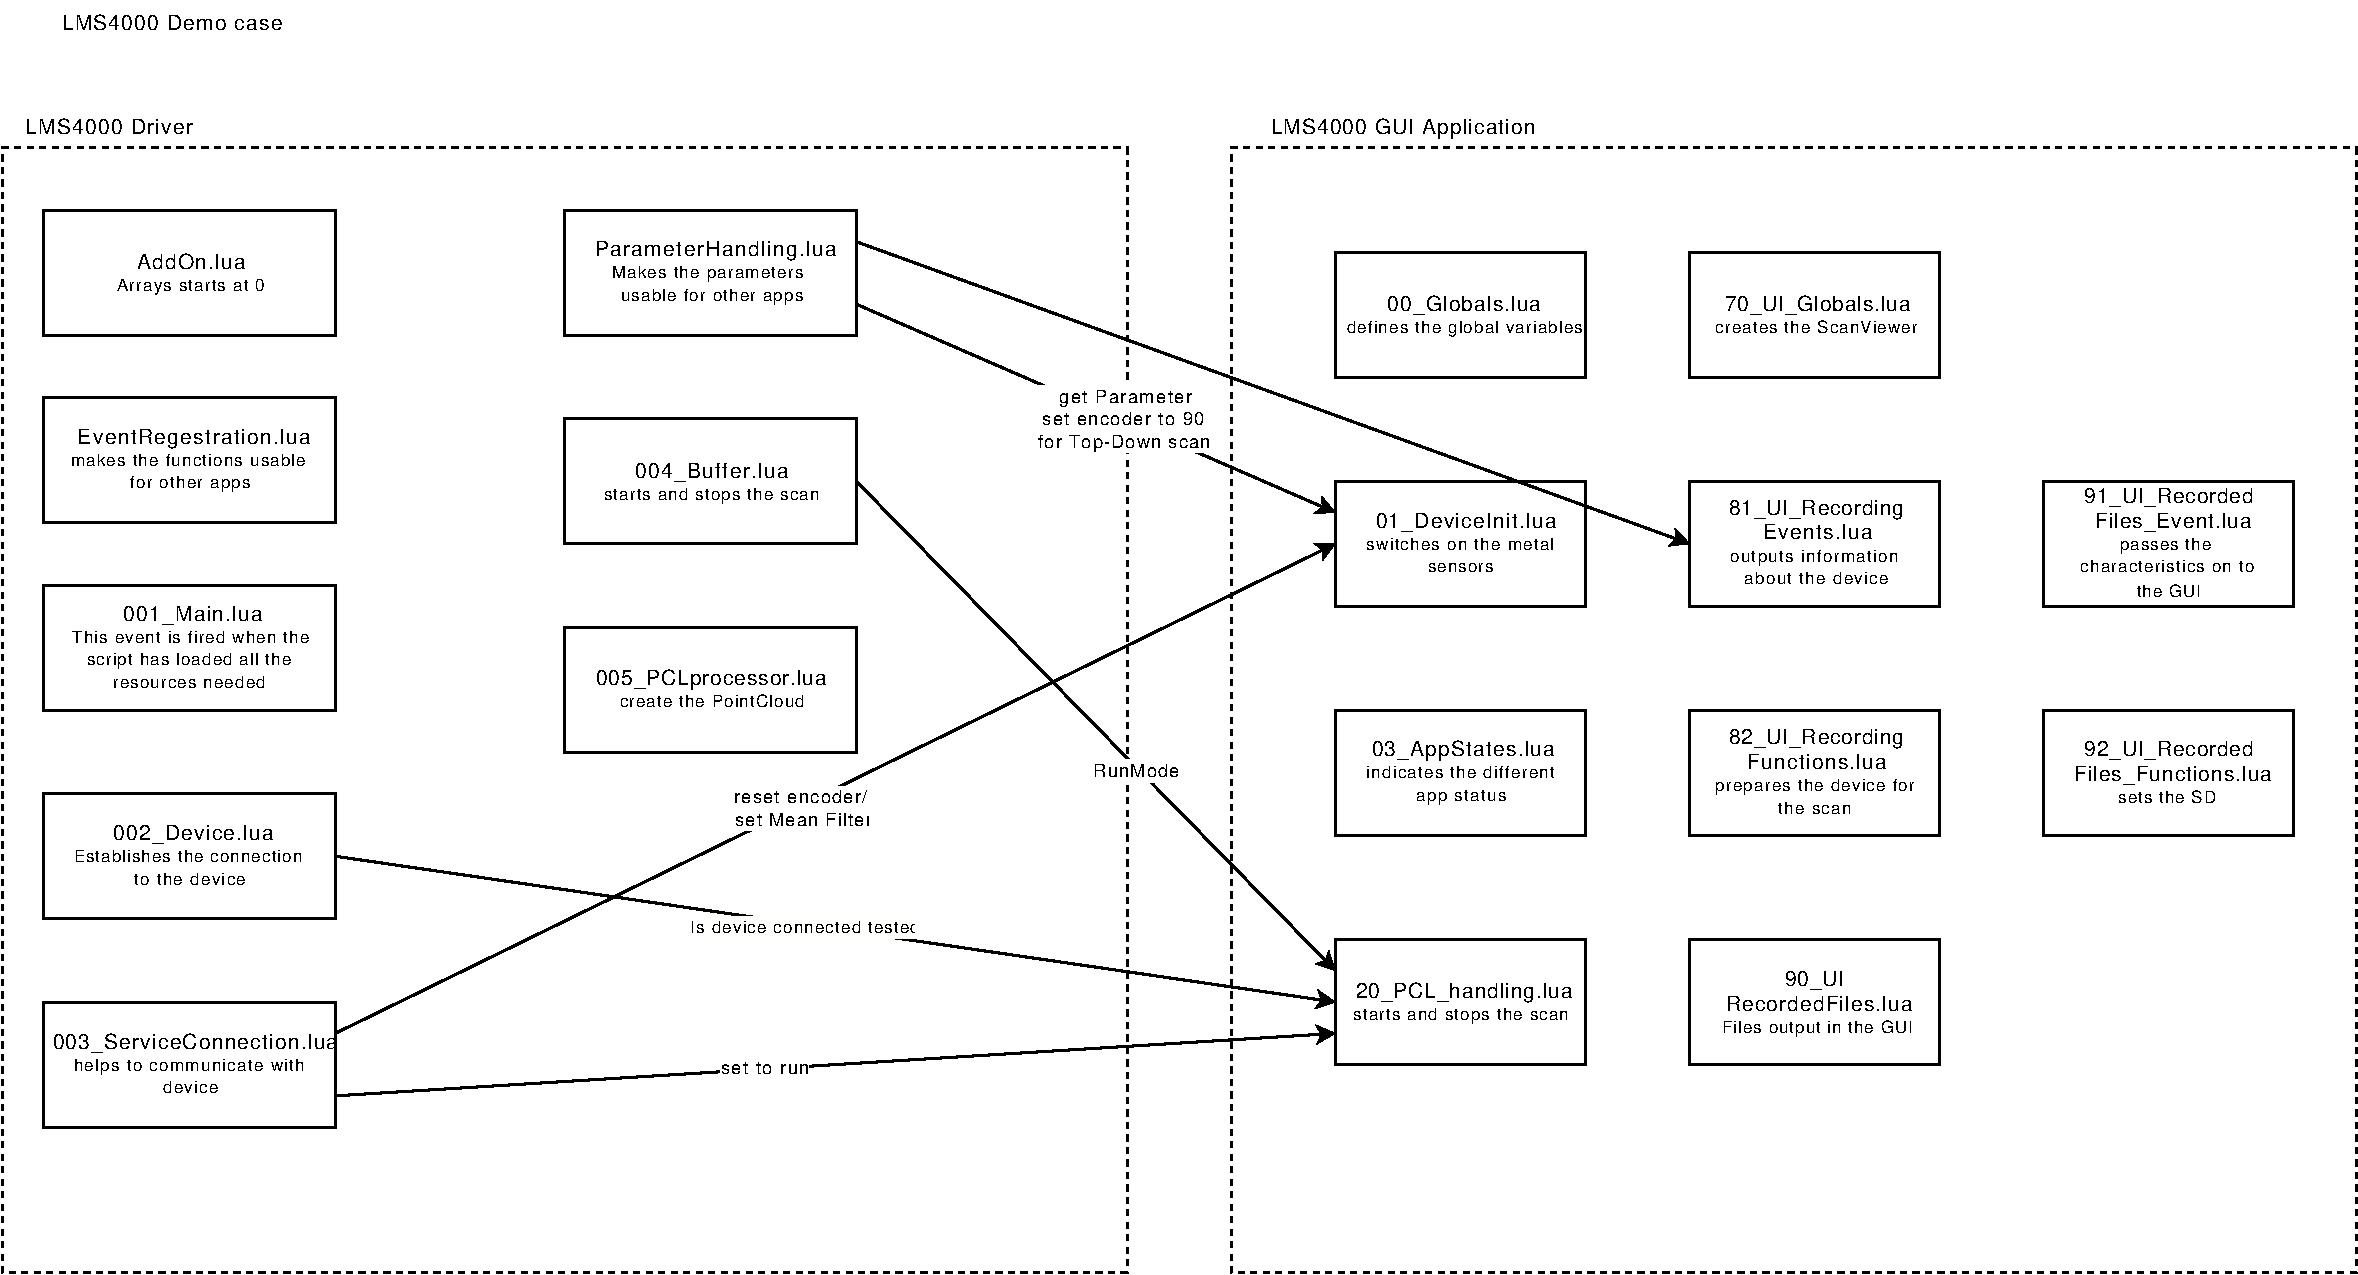
\includegraphics[width=15cm]{Bilder/SW - LMS4000 Democase (1).pdf}
\caption{Softwarearchitektur der Demokoffer App}
\label{Softwarearchitektur der Demokoffer App}
\end{figure}


\section{Neugestaltung der GUI}
\section{Behebung des Überlauf des Encoders}
